\chapter{Informatyka afektywna}
\label{cha:affectiveComputing}

Informatyka afektywna (ang. \textit{affective computing}) jest dziedziną informatyki, w której obliczenia są powiązane z emocjami, lub bezpośrednio na nie wpływają~\cite{Picard:1997:AC:265013}. Głównym celem informatyki afektywnej jest rozpoznawanie oraz analiza emocji ludzkich, możliwość ich symulacji przez komputer, a także wpływanie na emocje użytkownika poprzez konkretne bodźce. Aby uzyskać taki efekt, informatyka afektywna jest silnie powiązana z dziedzinami takimi jak psychologia, fizjologia, czy kognitywistyka~\cite{affective_computing_review_tao_tieniu}.

\section{Emocje}
Choć do dzisiaj nie ma jednej, uniwersalnej definicji czym są emocje, to środowisko naukowe ciągle przeprowadza badania na tematy powiązane z emocjami. Już w XIX wieku powstała teoria opracowana niezależnie przez Williama Jamesa oraz Carla Lange'a, w której emocję zdefiniowano jako interpretację reakcji cielesnej na zaobserwowany bodziec~\cite{Coleman2011}. Obaj badacze przyjęli, że na konkretny czynnik człowiek reaguje najpierw reakcją fizjologiczną, która następnie zostaje przez niego przypisana do wzorca odpowiadającego danej emocji. Dla przykładu, jeśli człowiek znajdzie się w sytuacji, w której zobaczy zagrożenie, zaczyna się trząść i~pocić, a jego tętno gwałtownie wzrasta, jego mózg natomiast interpretuje to jako strach.

Teoria Jamesa-Lange'a została zakwestionowana w latach dwudziestych XX wieku przez dwójkę naukowców, Waltera Cannona i~Phillipa Barda. Zasugerowali oni, że odczuwanie emocji nie jest zależne od reakcji fizjologicznych, a raczej są to reakcje zachodzące jednocześnie jako odpowiedź na dany bodziec~\cite{cannon_1927}. Teoria ta była bezpośrednim zakwestionowaniem badań przeprowadzonych przez Jamesa i~Lange'a. Jej autorzy przeprowadzili badania na kotach, na podstawie których przedstawili, że to wzgórze jest obszarem mózgu odpowiedzialnym za reakcje emocjonalne na doświadczane bodźce. Cannon zauważył, że całkowite odcięcie wszystkich układów od mózgu nie zmienia zachowania emocjonalnego zwierząt, co kłóciło się z teorią Jamesa-Lange'a, według której koty powinny przestać wykazywać jakiekolwiek reakcje emocjonalne.

\begin{figure}[h]
	\centering
	\begin{subfigure}{0.7\textwidth}
		
\includegraphics[width=\linewidth]{images/james-lang.png}
		\label{fig:james}
		\caption{Teoria Jamesa-Lange'a, źródło - opracowanie własne na podstawie~\cite{Coleman2011}}
	\end{subfigure}
	\begin{subfigure}{0.7\textwidth}
		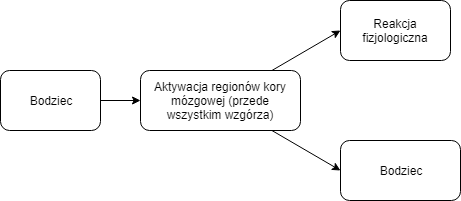
\includegraphics[width=\linewidth]{images/cannon-bard.png}
		\label{fig:canon}
		\caption{Teoria Canona-Barda, źródło - opracowanie własne na podstawie~\cite{cannon_1927}}
	\end{subfigure}
	\caption{Graficzne porównanie teorii emocji Jamesa-Lange'a i Canona-Barda}
\end{figure}

Teoria Jamesa-Lange'a została ponownie podjęta przez Prinza, który przedstawił więcej dowodów na potwierdzenie tej teorii, jednocześnie opisując argumenty pokazujące, że reakcje fizjologiczne nie zawsze są wystarczające, lub w ogóle niepotrzebne do odczuwania emocji~\cite{Prinz2004-PRIEE-2}. Zwrócił on między innymi uwagę na badania Hohmanna nad pacjentami z urazami rdzenia kręgowego~\cite{Hohmann1966SomeEO}, w których zauważono efekty zarówno potwierdzające, jak i podające w wątpliwość teorię Jamesa-Lange'a. Hohmann zauważył, że u osób z urazem można zauważyć redukcję w odczuwaniu emocji, ale niektóre z nich wciąż były zauważalne. Prinz komentuje to jako zdolność mózgu do przewidzenia reakcji fizjologicznej na dany bodziec, co z kolei będzie skutkować odczuwaniem emocji. Jest to możliwe dzięki wcześniejszym doświadczeniom. Tak jak człowiek, który stracił wzrok, jest w stanie wyobrazić sobie przedmiot, który kiedyś widział, tak samo mózg potrafi określić jaka reakcja fizjologiczna mogła nastąpić na dany bodziec.

\section{Pętla afektywna}
\url{https://www.researchgate.net/publication/220962601_Affective_Loop_Experiences_-_What_Are_They/link/0deec530769158251e000000/download}
Co to jest pętla afektywna, jaki jest schemat pętli

\section{Modele emocji}
Jakie mogą być modele, model russela, affective grid



\section{Gry z pętlą afektywną}
Jakie mogą być mechaniki (krótko), przykłady takich gier (proste - gry z wyborem wpływającym na rozgrywkę, złożone - Nevermind, Bring to Light)

\url{https://www.researchgate.net/profile/Eva_Hudlicka/ publication/228622615_Affective_computing_for_game_design/links/02bfe50e1936ab5b93000000/Affective-computing-for-game-design.pdf/}

\url{https://www.gamesradar.com/horror-game-nevermind-uses-biometrics-sense-your-fear/}

\url{https://store.steampowered.com/app/636720/Bring_to_Light/}


